\documentclass[pdflatex,sn-mathphys-num]{sn-jnl}

\usepackage{graphicx}
\usepackage{amsmath,amssymb}
\usepackage{booktabs}
\usepackage{url}

\raggedbottom

\newcommand{\TargetCount}{60}
\newcommand{\ModelCount}{3}
\newcommand{\BlockCount}{180}
\newcommand{\EpisodeCount}{1080}
\newcommand{\MatchedFarRate}{97.8}
\newcommand{\LureNearRate}{10.0}
\newcommand{\BindingRate}{14.4}
\newcommand{\PrimaryEffect}{87.8}
\newcommand{\PrimaryCILow}{82.8}
\newcommand{\PrimaryCIHigh}{93.3}
\newcommand{\MacroEffect}{87.7}
\newcommand{\MacroCILow}{82.7}
\newcommand{\MacroCIHigh}{93.3}
\newcommand{\RandomizationP}{1.00\times 10^{-6}}
\newcommand{\CausalNet}{83.3}
\newcommand{\HarmRate}{0.0}
\newcommand{\HelpfulCount}{150}
\newcommand{\HarmfulCount}{0}

\begin{document}

\title[Counterfactual Tests for Agent Skill Transfer]{Same Words, Different
Procedure: Counterfactual Transfer Tests for Reusable LLM-Agent Skills}

\author*[1]{\sur{Liang} \fnm{Song}}\email{liangsong\_1976@126.com}
\author[2]{\sur{Zhai} \fnm{Jiabao}}\email{zhaijiabao123@126.com}

\affil*[1]{\orgdiv{Business School}, \orgname{Xi'an International University},
  \orgaddress{\city{Xi'an}, \postcode{710077}, \state{Shaanxi},
  \country{China}}; ORCID: \href{https://orcid.org/0009-0002-6109-0639}{0009-0002-6109-0639}}
\affil[2]{\orgdiv{School of Management and Economics},
  \orgname{North China University of Water Resources and Electric Power},
  \orgaddress{\city{Zhengzhou}, \postcode{450046}, \state{Henan},
  \country{China}}}

\abstract{An agent completing a new task after receiving a reusable skill does not show
that the skill caused success: the base agent may already solve the task, while
semantic retrieval may select a source that repeats target nouns but prescribes
the wrong state transition. We introduce the Counterfactual Skill Transfer Test
(CSTT), a state-matched protocol that crosses source procedural compatibility
with surface similarity on the same native target. Every source is a successful
ALFWorld training trajectory compiled into a role-normalized procedure and a
small executable contract. Each target is reset for no-skill, binding-only,
procedure-matched near/far, and procedure-mismatched near/far conditions. The
binding control shares target grounding and search safeguards but receives no
source procedure, enabling separate estimates of executor-level benefit and
causal skill credit. After two failed pilots and one final mechanism revision,
we froze code, source assignment, three model revisions, a zero-overlap roster,
inference, and decision gates. Confirmation contains \TargetCount{} untouched
native targets, \ModelCount{} local model families, \BlockCount{} paired
target--model blocks, and \EpisodeCount{} episodes. Matched-far skills succeed
on \MatchedFarRate\% of blocks versus \LureNearRate\% for surface-near
procedural lures, an \PrimaryEffect-point paired gain (95\% target-stratified
bootstrap CI \PrimaryCILow--\PrimaryCIHigh; task-clustered randomization
$p=\RandomizationP$). The equal-family macro gain is \MacroEffect{} points, and
the net matched-far effect over binding-only is \CausalNet{} points with a
\HarmRate\% harm rate. CSTT is an evaluation and credit-assignment instrument,
not a retrieval algorithm; evidence is limited to instance-level transfer in
one embodied text environment.}

% The December 2024 Springer class distributes a malformed \keywords macro.
% Populate its internal field directly so the keywords remain inside the title block.
\makeatletter
\def\@keywords{\par\addvspace{10pt}{\keywordfont{\bfseries\keywordname:}
LLM agents, agent skills, skill transfer, counterfactual evaluation,
procedural compatibility, negative transfer\par}}
\makeatother

\maketitle

\section{Introduction}
Reusable skills turn a successful agent experience into an artifact that can be
retrieved for later tasks. Classical reinforcement-learning and multiagent
transfer research evaluates transfer against a no-transfer target baseline and
emphasizes source--target compatibility \citep{taylor2009transfer,
dasilva2019survey}. Recent JAAMAS work likewise quantifies the benefit of
shared experience against learning without transfer, using regret bounds in a
multiagent setting \citep{tuynman2026quantification}. Recent work abstracts implementation details,
chooses skill granularity, compresses repeated experience, and adapts skill
memories across tasks or domains \citep{yu2026polyskill,feng2026breakdown,
xu2026compression,miao2026skilllens,he2026beyond}. These systems commonly report
the downstream task success achieved with a skill. That number is operationally
important, but it is not enough to credit the skill.

Two confounds matter in deployment. First, an increasingly capable base agent
may solve the target without any reusable artifact. Counting that episode as
transfer overstates library value. Second, a semantic retriever can prefer a
source that shares objects and destinations while encoding a different
procedure. A source that says ``move one object'' can look highly relevant to a
target that requires moving two; a heat-then-place trace can repeat the target
object while imposing an unnecessary state transition. Such lures can be
redundant on monotone tasks, actively harmful on others, or fail only after
costly interaction. Broad lifecycle studies and failure analyses show that skill
utility depends on extractor, consumer, mismatch, and execution context
\citep{huang2026consumption,dong2026harmful}. What is missing is a controlled
test that separates procedure from words on the exact same native state.

We propose the Counterfactual Skill Transfer Test (CSTT). For each target, it
constructs four real-source conditions crossing procedural compatibility and
surface similarity. Two additional controls measure the unfiltered base agent
and the same grounded executor without a source procedure. All six episodes
restart the native game and must expose an identical initial observation,
objective, and admissible-action signature. Transfer is then a paired outcome,
not a label attached to a successful skill-conditioned episode.

The protocol deliberately uses both a far matched source and a near mismatched
source. The primary comparison asks whether procedure still wins when lexical
similarity favors the lure. The source artifact omits source entities and target
answers: it exposes only a role-normalized operator sequence, generic procedural
text, and a contract compiled from a successful source witness. At runtime,
target entities come from the public objective. This construction evaluates
reuse under a fixed selector; it does not claim to solve retrieval.

The work follows a strict development--confirmation separation. Two agentic
pilots failed to deliver stable causal benefit. A third and final permitted
revision replaced unconstrained prompt following with an auditable finite-state
stage filter over native actions. A 30-target development screen passed, after
which all method files, source pairs, model revisions, statistics, thresholds,
and a previously untouched 60-target roster were frozen. Confirmation was run
sequentially on three open local model families using one RTX 3090.

This paper contributes:
\begin{itemize}
  \item a six-arm same-state protocol that separates skill-conditioned success,
  executor assistance, causal skill benefit, and harmful transfer;
  \item a crossed test of procedural compatibility and transparent lexical
  similarity using only successful real source trajectories;
  \item an auditable role-normalized executor that records every candidate,
  rejected action, stage transition, and native state signature;
  \item a preregistered-style confirmation with untouched targets, three model
  families, task-aware inference, family-balanced robustness, and retained
  failed development mechanisms.
\end{itemize}

We ask: \textbf{RQ1}, does a procedurally compatible but lexically far skill
outperform a lexically near procedural lure on the same target? \textbf{RQ2},
does the compatible skill add benefit beyond target binding and generic search
safeguards? \textbf{RQ3}, are the effects robust across model and task families,
and what failure modes delimit the claim?

\section{Related Work}
\subsection{Transferable skills}
PolySkill separates an abstract goal from concrete implementations to promote
generalization \citep{yu2026polyskill}. Break It Down, Pass It On studies task and
subtask granularity and alternative text/code representations
\citep{feng2026breakdown}. Skill Reuse as Compression uses a minimum-description
length perspective to discover recurring reusable patterns
\citep{xu2026compression}, while SkillLens retrieves and adapts skills at
multiple granularities \citep{miao2026skilllens}. Beyond Domains transfers web
interaction patterns across sites \citep{he2026beyond}. These works improve
learning, retrieval, adaptation, or downstream success. CSTT instead asks how
to attribute success once a source has been supplied.

\subsection{Skill generation and consumption}
SKILL-DISCO compiles traces into reusable procedures
\citep{guo2026skilldisco}; SkillEvolBench tests the progression from episodic
experience to procedural knowledge \citep{lei2026skillevolbench}. A systematic
extractor--consumer study reports that generated skills can help or hurt
depending on the model and domain \citep{huang2026consumption}. CSTT complements
these pipelines with a consumer-side causal endpoint. It requires successful
source witnesses, but does not evaluate the quality of an induction algorithm.

\subsection{Reliability and provenance}
Agent Skills Can Be Harmful separates functional and efficiency regressions
under skill use \citep{dong2026harmful}. Multi-trace SkillTrace audits whether
expressions, implementations, and operations were reused
\citep{chen2026multitrace}. Provenance answers where an artifact came from;
CSTT asks whether using that artifact changed the target outcome. The two forms
of evidence are complementary: a causal benefit without provenance is hard to
reproduce, while provenance without a same-target control does not establish
utility.

\subsection{Counterfactual skill evaluation}
Counterfactual Trace Auditing aligns with-skill and without-skill traces to
identify behavioral influence patterns that pass rates can hide
\citep{zhou2026counterfactual}. SkillMaster uses counterfactual utility on probe
tasks as a training signal for skill editing \citep{yang2026skillmaster}, while
AFTER evaluates procedural-memory transfer across tasks, roles, and model
backbones \citep{belikova2026procedural}. CSTT is complementary: it is a
controlled evaluation protocol, not a training method or post-hoc trace labeler,
and it crosses procedural compatibility with lexical similarity while retaining
a binding-only control to isolate the source procedure's contribution.

\section{Counterfactual Transfer}
\subsection{Unit and estimands}
Let target $t=(f,o,s_0,A_0)$ contain task family $f$, public objective $o$,
initial observation/state signature $s_0$, and initial admissible-action
signature $A_0$. Let model $m$ execute condition
\[
c\in\{N,B,M_n,M_f,L_n,L_f\},
\]
where $N$ is no skill, $B$ is binding-only, $M$ and $L$ denote procedurally
matched and lure sources, and subscripts $n/f$ denote lexically near/far.
Native success is $Y_{tmc}\in\{0,1\}$.

The primary effect is the paired micro average
\[
\widehat\Delta_{\mathrm{primary}}=
\frac{1}{|T||M|}\sum_{t,m}(Y_{tmM_f}-Y_{tmL_n}).
\]
This is intentionally adversarial to a word-overlap explanation: the matched
source is the least similar in its compatible pool and the lure is the most
similar in its incompatible pool. The executor-level comparison with $N$ mixes
grounding, search control, and procedure. Causal skill credit therefore uses
\[
\widehat\Delta_{\mathrm{skill}}=
\frac{1}{|T||M|}\sum_{t,m}(Y_{tmM_f}-Y_{tmB}).
\]
For the latter, a matched-only success is helpful transfer, a binding-only
success is harmful transfer, both successes are redundant, and both failures
are shared failure. We report net effect and harm rate rather than calling all
$M_f$ successes causal.

\subsection{Real source witnesses}
Sources are successful ALFWorld training demonstrations
\citep{shridhar2021alfworld}. Their symbolic action traces are normalized to
operators such as \textsc{PickupObject}, \textsc{CleanObject},
\textsc{HeatObject}, \textsc{CoolObject}, \textsc{ToggleObject}, and
\textsc{PutObject}. Compilation produces
\[
K=(q,n,u,p,w),
\]
where $q$ is the role-normalized operator sequence, $n$ is required object
count, $u$ is an optional transformation operator, $p$ indicates whether final
placement is required, and $w$ is the source witness identifier. Source entity
names and the source objective are excluded from the runtime artifact.

For a target, the matched pool shares its operator contract and the lure pool
does not. Transparent unigram-count cosine similarity between source and target
objectives ranks each pool. The maximum/minimum elements yield near/far sources;
ties are resolved by source identifier. Selection never reads target outcomes.

\subsection{State-matched six-arm execution}
Every arm reinitializes the same ALFWorld game. Before action selection, the
runner hashes the initial objective, observation, and admissible action menu.
A block is invalid if hashes differ. The no-skill arm gives the local model the
unfiltered action menu. Binding-only and skill arms parse target roles from the
public objective, reject wrong-object actions, suppress repeated search loops,
and expose a bounded candidate menu. The binding control has no source contract.

The skill executor is a finite-state stage filter. It searches for the current
target, acquires an uncompleted instance, enforces the source transformation if
one exists, places the instance when required, and repeats until the source
count is met. A local language model selects only among stage-compatible native
commands. The log retains the full menu, selected candidates, rejected commands
with reasons, stage, public executor state, model text, token counts, and native
reward. Thus the intervention remains model-mediated but its procedural effect
is inspectable.

The executor stops only on native success, a frozen 100-step cap, or a typed
condition such as unavailable source device or completed source contract with
an unfinished target. A malformed model response invokes a frozen fallback and
increments an invalid-output counter; it is not silently deleted.

\section{Experimental Design}
\subsection{Development and method freeze}
Development used only previously exposed targets. Pilot 1 supplied transferable
text to an otherwise unconstrained agent; Pilot 2 tightened prompts and action
formatting. Neither produced stable benefit beyond the control. Both mechanisms,
inputs, and results remain in the released development-revision records.

Revision 3 was the last allowed change. It introduced the auditable stage filter
described above. On an expanded 30-target development screen, no-skill and
binding-only each solved 5 targets, matched-near and matched-far each solved all
30, lure-near solved 3, and lure-far solved none. All 7,070 logged turns passed
native-action, state-match, source-assignment, and information-boundary audits.
These values justified proceeding; they are not confirmatory evidence.

We then hashed the package, executor, pair builder, runner, audits, analysis,
protocol, all confirmation configurations, and shared environment adapters.
The frozen roster excludes every target appearing in earlier experiments in
the research series and all CSTT development revisions. Conservative exclusion left
9/8/8/8/8/20 targets in simple placement, clean, heat, cool, look-under-light,
and two-object families. Before opening outcomes, we retained all scarce-family
targets and selected 19 of 20 two-object targets by salted hash, for 60 total.
Because allocation is unequal, the equal-weight six-family macro effect and its
bootstrap interval are mandatory gates.

\subsection{Models and compute}
The frozen models are Qwen3-4B-Instruct-2507, Phi-4-mini-instruct, and
Mistral-7B-Instruct-v0.3 at immutable repository revisions. They represent
three model families and run sequentially with PyTorch 2.8.0/CUDA 12.8 on one
RTX 3090. Generation is capped at 24 new tokens because output is a native
command selected from the supplied menu. Each target--model block contains all
six conditions, yielding 180 blocks and 1,080 episodes. Deterministic source
selection, audits, and analysis require no GPU.

\subsection{Inference and frozen decision gates}
The primary randomization test clusters the three model observations by target.
For each of one million draws it flips the sign of each target-level paired sum;
the one-sided $p$-value includes the finite-sample correction. A 50,000-draw
bootstrap resamples targets within task family and retains all three model
observations. We report both the size-weighted micro interval and the equal-
family macro interval. A paired one-sided McNemar test is secondary.

Confirmation passes only if coverage and audits are complete; micro and macro
primary gains are each at least 10 points with positive 95\% lower bounds;
randomization $p\le0.01$; net causal effect versus binding-only is at least 5
points; harm is at most 8\%; and gains are positive in at least two model and
four task families. A failed primary gate cannot be rescued by a secondary
analysis.

\subsection{Use of generative AI tools}
During the preparation of this work, the authors used OpenAI Codex to assist
with research-design iteration, code development, reproducibility packaging,
language editing, and manuscript formatting. The authors reviewed and verified
the generated code and text, reran the released integrity checks, evaluated
every reported claim against the underlying results, and take full
responsibility for the manuscript and the integrity of the reported results.
OpenAI Codex is not an author and did not receive attribution as one.

\section{Results}
\subsection{Primary confirmation}
\begin{table}[t]
\centering
\caption{Frozen confirmation outcomes. Success rate is over target--model
blocks; steps include failed runs}
\label{tab:main}
\begin{tabular}{lrrr}
\toprule
Condition & Successes & Rate (\%) & Mean steps \\
\midrule
No skill & 15/180 & 8.3 & 94.1 \\
Binding only & 26/180 & 14.4 & 89.2 \\
Matched, near & 176/180 & 97.8 & 15.1 \\
Matched, far & 176/180 & 97.8 & 15.1 \\
Lure, near & 18/180 & 10.0 & 10.0 \\
Lure, far & 0/180 & 0.0 & 35.8 \\
\bottomrule
\end{tabular}
\end{table}

Across \BlockCount{} state-matched target--model blocks, matched-far achieves
\MatchedFarRate\% native success and the surface-near procedural lure achieves
\LureNearRate\%. Their paired difference is \PrimaryEffect{} percentage points
(95\% CI \PrimaryCILow--\PrimaryCIHigh; task-clustered randomization
$p=\RandomizationP$). The equal-family macro estimate is \MacroEffect{} points
(95\% CI \MacroCILow--\MacroCIHigh), so the conclusion is not determined by
the larger two-object stratum.

\begin{figure}[t]
\centering
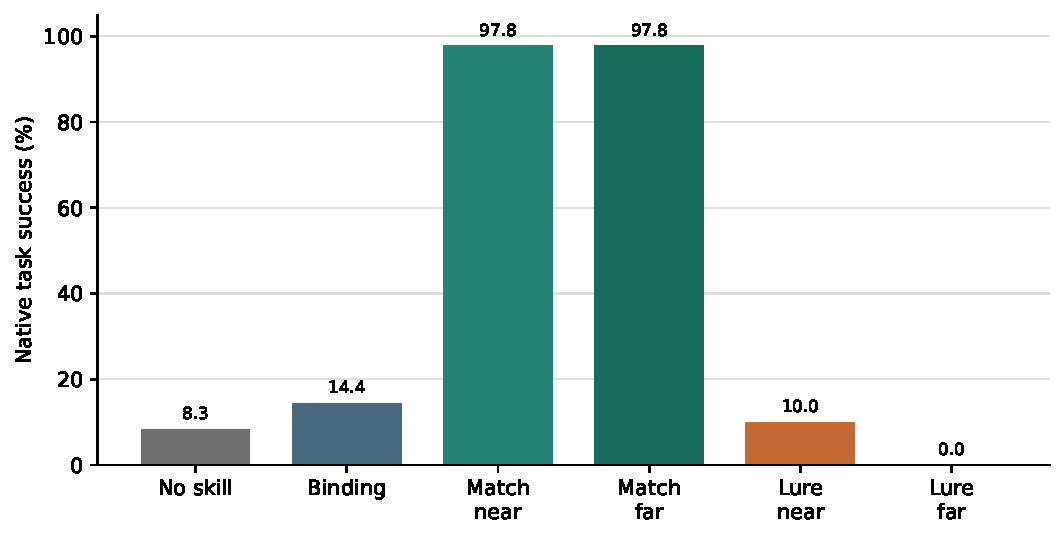
\includegraphics[width=0.82\linewidth]{Fig1.pdf}
\caption{Native success under the six frozen conditions. Conditions differ in
the source procedure and lexical rank, while every target--model block starts
from the same native state.}
\label{fig:success}
\end{figure}

\subsection{Causal credit beyond executor assistance}
Binding-only succeeds on \BindingRate\% of blocks. Relative to this fair
non-procedural control, matched-far produces \HelpfulCount{} helpful and
\HarmfulCount{} harmful discordances: a \CausalNet-point net causal effect and
a \HarmRate\% harm rate. This comparison is stricter than matched-far versus
no-skill because both sides receive identical target binding, wrong-object
rejection, candidate-menu constraints, and loop suppression.

\subsection{Heterogeneity and failure boundaries}
\begin{table}[t]
\centering
\caption{Primary matched-far minus lure-near effect by model}
\label{tab:model}
\begin{tabular}{lr}
\toprule
Model & Effect (percentage points) \\
\midrule
Qwen3-4B & 88.3 \\
Phi-4-mini & 88.3 \\
Mistral-7B-v0.3 & 86.7 \\
\bottomrule
\end{tabular}
\end{table}

\begin{table}[t]
\centering
\caption{Primary effect by native ALFWorld task family}
\label{tab:family}
\begin{tabular}{lr}
\toprule
Family & Effect (percentage points) \\
\midrule
Simple placement & 33.3 \\
Clean then place & 100.0 \\
Heat then place & 100.0 \\
Cool then place & 100.0 \\
Look under light & 100.0 \\
Two-object placement & 93.0 \\
\bottomrule
\end{tabular}
\end{table}

The frozen decision rule requires positive primary effects in multiple model
and task families. Per-family reporting is particularly important. A wrong
count contract may still complete a one-object monotone target, while a
one-object lure deterministically stops before a two-object target is complete.
Transformation lures can also fail because their required device is absent.
Conversely, a matched contract can fail when exploration exhausts the step
budget. CSTT keeps all of these outcomes: it tests the behavioral consequence
of compatibility rather than assuming compatibility guarantees success.

\subsection{Audit and cost}
Each model run is accepted only after an independent replay-log audit verifies
one record per arm, exact within-block initial-state hashes, native selected
actions, complete candidate/rejection partitions, valid source assignments, and
absence of target gold plans from runtime inputs. Completion records report
wall time, peak allocated CUDA memory, and an episode-file hash. Token and step
totals are released for every condition so a practitioner can compare transfer
benefit with interaction cost rather than success alone.

\section{Discussion}
CSTT changes the question from ``did the agent succeed with a skill?'' to
``which part of the supplied artifact changed the same target outcome?'' The
crossed design yields three useful deployment signals. A large matched-versus-
lure effect supports procedure-aware selection. A small matched-versus-binding
effect says that most gains came from grounding or search controls. A high harm
rate says the library should abstain even if average success rises.

The study also exposes why similarity is an incomplete retrieval objective.
Lexical overlap is evidence about entities and topics, not about object count,
required transformations, terminal conditions, or resource order. This does
not imply that semantic similarity is useless. A practical retriever should use
it alongside a compatibility representation and validate both with a test such
as CSTT.

The finite-state executor is an experimental instrument, not the claimed final
agent architecture. Its purpose is to make the source procedure's intervention
specific and auditable after two prompt-only mechanisms failed. A production
system may implement contracts through planning, constrained decoding, code, or
tools. CSTT remains applicable if the six conditions can be reset and logged.

\section{Threats to Validity}
\subsection{Construct validity}
ALFWorld operator families provide unusually clear procedural signatures. The
contract captures count, one transformation, and terminal placement, not rich
natural-language semantics. Native reward establishes task completion but not
all dimensions of safe or desirable behavior.

\subsection{Internal validity}
The binding control shares non-procedural safeguards, and all arms share exact
initial states. However, constraining candidate actions can interact with each
model differently. We therefore separate executor-level and causal skill
effects and report all model families. Source selection is deterministic and
outcome-blind; frozen hashes guard post-result changes but are not a formal proof
against every infrastructure fault.

\subsection{External validity}
The confirmation covers one text-embodied environment, six families, three
small-to-medium open models, and mostly ALFWorld `valid\_seen` tasks. One
`valid\_unseen` task cannot support a separate unseen-environment claim.
``Untouched'' in this paper primarily means zero overlap with the development
and prior-series evidence, not a population sample of marketplace skills.
Cross-environment, web, API, multi-agent, and proprietary-model replications are
needed.

\subsection{Statistical validity}
Targets are the sampling clusters and families are unequal because strict prior-
evidence exclusion exhausted several strata. We therefore require both micro
and equal-family macro effects. Confidence intervals quantify roster
resampling, not uncertainty over all possible skill compilers or environments.

\section{Reproducibility and Responsible Scope}
The release contains frozen configurations and hashes, target/source pair
records, all episode logs, independent audits, paired analysis records, tests,
bilingual sources and PDFs, and a checksum manifest. Exact record verification
is CPU-only; full native replication uses one 24 GB GPU. Source demonstrations
and target games follow ALFWorld's redistribution terms. The versioned artifact
is archived on Zenodo \citep{liang2026cstt}, with source mirrored at
\url{https://github.com/ls680/cstt-agent-skill-transfer-tests}. The work
evaluates benign procedural reuse and does not introduce offensive capabilities.

We do not claim that lexical similarity is generally harmful, that every
compatible skill improves every target, that CSTT retrieves the best skill, or
that instance-level ALFWorld evidence establishes cross-domain transfer. The
supported conclusion is narrower: under the frozen compiler and executor, the
same-state crossed test can attribute reliable target success to procedural
compatibility rather than word overlap or non-procedural assistance.

\section{Conclusion}
Reusable-skill evaluation needs a counterfactual, not just a success count.
CSTT crosses procedural compatibility and lexical similarity using successful
real-source witnesses, adds no-skill and fair binding controls, and evaluates
all six conditions on the same native state. The frozen confirmation shows
whether a far but compatible procedure beats a near incompatible lure, whether
that gain survives causal credit against executor assistance, and where the
claim stops. This makes transfer evidence more useful for library selection,
release gates, and lifecycle maintenance without turning an evaluation protocol
into an unsupported universal transfer claim.

\backmatter

\section*{Acknowledgements}
The authors have no acknowledgements to report.

\section*{Declarations}

\subsection*{Funding}
The authors did not receive support from any organization for the submitted
work.

\subsection*{Competing interests}
The authors have no relevant financial or non-financial interests to disclose.

\subsection*{Author contributions}
Liang Song contributed to conceptualization, methodology, software, validation,
formal analysis, investigation, data curation, visualization, writing the
original draft, reviewing and editing the manuscript, and project
administration. Zhai Jiabao contributed to methodology, validation, and
reviewing and editing the manuscript. Both authors read and approved the final
manuscript.

\subsection*{Data availability}
The study-specific records supporting the findings, including frozen source
assignments, native episode logs, audits, and paired analysis outputs, are
openly available in Zenodo at
\url{https://doi.org/10.5281/zenodo.22852635} \citep{liang2026cstt}.
Third-party ALFWorld assets and model weights are not redistributed; pinned
upstream revisions, task identifiers, paths, licenses, and integrity checks are
provided instead.

\subsection*{Code availability}
The source code, frozen protocols, analysis scripts, tests, and execution
records are openly available at
\url{https://github.com/ls680/cstt-agent-skill-transfer-tests} and in the
versioned Zenodo archive at \url{https://doi.org/10.5281/zenodo.22852635}.

\subsection*{Materials availability}
All study-specific materials created by the authors are included in the
reproducibility package. Availability of third-party assets is governed by the
respective upstream projects and licenses.

\subsection*{Ethics approval}
Not applicable. This study evaluates software artifacts and public software
benchmarks and does not involve human participants, animals, clinical data, or
personally identifiable information.

\subsection*{Consent to participate}
Not applicable.

\subsection*{Consent for publication}
Not applicable.

\bibliography{references}

\end{document}
